% Capítulo 7. Resultados y análisis de KPIs. Spec: ESQUEMA.md §4, capítulo 7.

Este capítulo compara el plan del modelo híbrido (la mejor solución encontrada, descrita en el capítulo~\ref{ch:implementacion}) con el caso base del capítulo~\ref{ch:caso-base}, sobre las mismas \RutasMuestra{} rutas y \CorridasMuestra{} corridas laborales. Todas las tablas muestran el cambio absoluto ($\Delta$) y porcentual ($\Delta\%$) respecto del caso base.

\section{Indicadores principales}
\label{sec:kpis-resultados}

El modelo cubre las mismas corridas con \BusesModelo{} buses, \DeltaBuses{} respecto del caso base (\DeltaPctBuses\,\%), y con un costo de USD~\CostoModelo{} al día, \DeltaPctCosto\,\% menos (Tabla~\ref{tab:kpis}). Los kilómetros en vacío bajan de \PctVacioBase\,\% a \PctVacioModelo\,\% del total, porque un bus del modelo puede tomar corridas de distintas rutas de su sector y encadenar la que empieza más cerca. La energía comprada cae casi a una décima, pero esa cifra no se puede leer sola: el caso base carga siempre hasta el 100\,\% y termina el día con mucha más energía en las baterías (sección~\ref{sec:energia}).

\begin{table}[htbp]
\centering
\caption{Indicadores del caso base y del modelo híbrido (\RutasMuestra{} rutas, día laboral).}
\label{tab:kpis}
\begin{tabular}{lrrrr}
\toprule
Indicador & Caso base & Modelo & $\Delta$ & $\Delta\%$ \\
\midrule
Buses utilizados & \BusesBase & \BusesModelo & \DeltaBuses & \DeltaPctBuses \\
Costo total (USD/día) & \CostoBase & \CostoModelo & \DeltaCosto & \DeltaPctCosto \\
Km en vacío (\% de los km) & \PctVacioBase & \PctVacioModelo & \DeltaPpVacio{} pp & --- \\
Energía comprada (kWh) & \EnergiaBase & \EnergiaModelo & \DeltaEnergia & \DeltaPctEnergia \\
Sesiones de carga & \SesionesBase & \SesionesModelo & \DeltaSesiones & \DeltaPctSesiones \\
\bottomrule
\end{tabular}
\end{table}

\section{Composición del costo}
\label{sec:composicion-costo}

La flota pesa lo mismo en ambos planes, \PctFlotaBase\,\% y \PctFlotaModelo\,\% del costo (Tabla~\ref{tab:costos}), y es la palanca principal: de los USD~\DeltaCosto{} de diferencia diaria, USD~\DeltaCostoFlota{} corresponden a los buses que el modelo deja de usar. Los kilómetros aportan USD~\DeltaCostoKm, por el menor recorrido en vacío. La electricidad y las sesiones pesan poco en el costo (\PctEnergiaModelo\,\% y \PctSesionesModelo\,\% en el modelo), pero cuándo y dónde se carga decide cuántos buses hacen falta: un bus que alcanza a cargar entre dos corridas no necesita un reemplazo.

\begin{table}[htbp]
\centering
\caption{Composición del costo diario (USD/día y porcentaje del costo total de cada plan).}
\label{tab:costos}
\small
\begin{tabular}{lrrrrrr}
\toprule
 & \multicolumn{2}{c}{Caso base} & \multicolumn{2}{c}{Modelo} & & \\
\cmidrule(lr){2-3}\cmidrule(lr){4-5}
Componente & USD & \% & USD & \% & $\Delta$ & $\Delta\%$ \\
\midrule
Flota & \CostoFlotaBase & \PctFlotaBase & \CostoFlotaModelo & \PctFlotaModelo & \DeltaCostoFlota & \DeltaPctCostoFlota \\
Kilómetros & \CostoKmBase & \PctKmBase & \CostoKmModelo & \PctKmModelo & \DeltaCostoKm & \DeltaPctCostoKm \\
Electricidad & \CostoEnergiaBase & \PctEnergiaBase & \CostoEnergiaModelo & \PctEnergiaModelo & \DeltaCostoEnergia & \DeltaPctCostoEnergia \\
Sesiones & \CostoSesionesBase & \PctSesionesBase & \CostoSesionesModelo & \PctSesionesModelo & \DeltaCostoSesiones & \DeltaPctCostoSesiones \\
\midrule
Total & \CostoBase & 100 & \CostoModelo & 100 & \DeltaCosto & \DeltaPctCosto \\
\bottomrule
\end{tabular}
\end{table}

\section{De dónde sale la diferencia}
\label{sec:etapas}

Para saber si la diferencia se debe a un caso base débil o al modelo, la Tabla~\ref{tab:etapas} sigue la solución etapa por etapa. La construcción cronológica (capítulo~\ref{ch:metodologia}), sin ninguna búsqueda local, ya ahorra \AhorroBusesConstruccion{} buses, el \PctAhorroConstruccion\,\% de la reducción total. Respecto del caso base, que también recarga, la construcción cambia tres cosas: los buses se comparten entre las rutas de un mismo sector, cada bus carga solo la energía que necesita en vez de llenar la batería, y cada corrida se asigna al bus disponible con el traslado en vacío más corto. Son decisiones de coordinación del modelo, no un efecto de que el caso base no cargue. La búsqueda local por parejas y tríos, con su refinamiento, aporta los \AhorroBusesBusqueda{} buses restantes. Como las etapas se aplicaron en secuencia, la tabla no aísla el efecto de cada regla por separado.

\begin{table}[htbp]
\centering
\caption{Buses y costo por etapa del método, comparados con el caso base.}
\label{tab:etapas}
\begin{tabular}{lrrrr}
\toprule
Etapa & Buses & Costo (USD/día) & $\Delta$ buses & $\Delta\%$ costo \\
\midrule
Caso base miope & \BusesBase & \CostoBase & --- & --- \\
Construcción cronológica & \BusesConstruccion & \CostoConstruccion & \DeltaBusesConstruccion & \DeltaPctCostoConstruccion \\
\quad + parejas & \BusesParejas & \CostoParejas & \DeltaBusesParejas & \DeltaPctCostoParejas \\
\quad + tríos & \BusesTrios & \CostoTrios & \DeltaBusesTrios & \DeltaPctCostoTrios \\
\quad + refinamiento (modelo) & \BusesModelo & \CostoModelo & \DeltaBuses & \DeltaPctCosto \\
\bottomrule
\end{tabular}
\end{table}

\section{Energía: cuándo y cuánto se carga}
\label{sec:energia}

La Figura~\ref{fig:energia} muestra la energía cargada según la hora del día, coloreada por la tarifa de esa hora. El caso base carga el \PctEnergiaPuntaBase\,\% de su energía en las horas de tarifa más alta (USD~\TarifaPunta{} por kWh), sobre todo al atardecer, cuando las baterías de los buses que partieron en la mañana se agotan. El modelo reparte la carga a lo largo del día y carga parte en la madrugada: solo el \PctEnergiaPuntaModelo\,\% de su energía se paga a la tarifa más alta, y el precio medio que paga baja de USD~\PrecioMedioKwhBase{} a \PrecioMedioKwhModelo{} por kWh.

\begin{figure}[htbp]
\centering
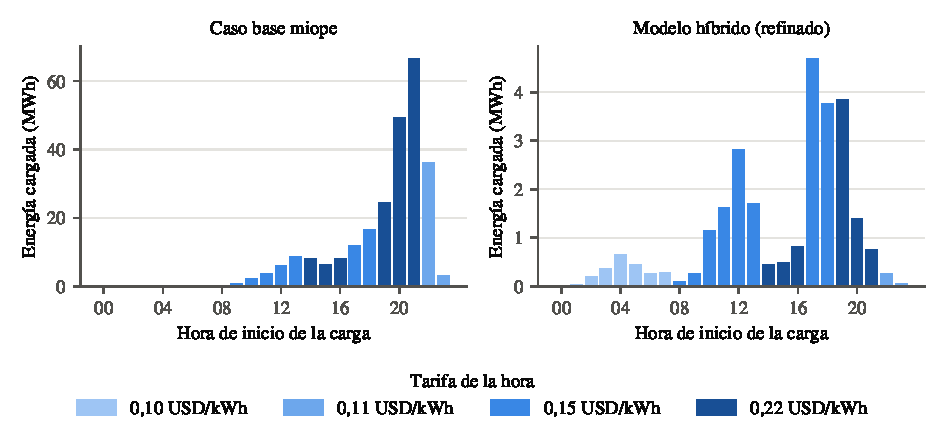
\includegraphics[width=\textwidth]{figures/energia_por_hora.pdf}
\caption{Energía cargada por hora de inicio de la carga, según la tarifa de esa hora. Cada panel tiene su propia escala: el caso base carga cerca de diez veces más energía que el modelo.}
\label{fig:energia}
\end{figure}

La energía comprada no es comparable directamente. Ambos planes parten con las baterías llenas y ninguno paga esa carga inicial, pero terminan con distinta energía: para volver a dejar llenos todos los buses, al caso base le faltan \DeficitBase~kWh y al modelo, \DeficitModelo~kWh. Si esa diferencia se valoriza a la tarifa nocturna de USD~\TarifaNocturna{} por kWh, el costo ajustado es de USD~\CostoAjustadoBase{} para el caso base y USD~\CostoAjustadoModelo{} para el modelo. La ventaja del modelo se reduce de \DeltaPctCosto\,\% a \DeltaPctCostoAjustado\,\%, pero se mantiene. Si esa energía alcanza a reponerse durante la noche es otra pregunta, que se analiza en el capítulo~\ref{ch:supuestos}.

\section{Uso de los electroterminales}
\label{sec:uso-electroterminales}

En el modelo, las plazas de los cinco electroterminales llegan a su capacidad, mientras que las conexiones de carga en uso simultáneo nunca pasan de unas pocas decenas (Tabla~\ref{tab:electroterminales}). El recurso que limita no son los cargadores, sino el espacio físico: los buses ocupan plazas mientras esperan su próxima corrida o al terminar su jornada. En el caso base, la ocupación máxima coincide con las conexiones en uso, porque sus buses solo entran al electroterminal para cargar. Para la entrega final, esto sugiere estudiar más plazas de estacionamiento o un mejor uso de los terminales de espera antes que más cargadores.

\begin{table}[htbp]
\centering
\caption{Ocupación máxima de plazas y conexiones de carga por electroterminal (cada uno tiene tantas conexiones como plazas).}
\label{tab:electroterminales}
\begin{tabular}{lrrrrr}
\toprule
 & & \multicolumn{2}{c}{Plazas ocupadas} & \multicolumn{2}{c}{Conexiones en uso} \\
\cmidrule(lr){3-4}\cmidrule(lr){5-6}
Electroterminal & Plazas & Caso base & Modelo & Caso base & Modelo \\
\midrule
E1 & \CapacidadEUno & \PlazasEUnoBase & \PlazasEUnoModelo & \ConexionesEUnoBase & \ConexionesEUnoModelo \\
E2 & \CapacidadEDos & \PlazasEDosBase & \PlazasEDosModelo & \ConexionesEDosBase & \ConexionesEDosModelo \\
E3 & \CapacidadETres & \PlazasETresBase & \PlazasETresModelo & \ConexionesETresBase & \ConexionesETresModelo \\
E4 & \CapacidadECuatro & \PlazasECuatroBase & \PlazasECuatroModelo & \ConexionesECuatroBase & \ConexionesECuatroModelo \\
E5 & \CapacidadECinco & \PlazasECincoBase & \PlazasECincoModelo & \ConexionesECincoBase & \ConexionesECincoModelo \\
\bottomrule
\end{tabular}
\end{table}

\section{Variabilidad de la búsqueda}
\label{sec:variabilidad}

La búsqueda local se detiene por tiempo de reloj, así que su resultado depende del presupuesto y del equipo. Para medir esa variabilidad se repitió la búsqueda desde la construcción con presupuestos de 15 a 240 segundos por etapa, tres veces cada uno, en un mismo equipo (Anexo~\ref{an:barrido}). La mediana del ahorro sobre la construcción sube de USD~\MedianaAhorroQuince{} al día (\MedianaBusesEvitadosQuince{} buses) con 15 segundos a USD~\MedianaAhorroDosCuarenta{} (\MedianaBusesEvitadosDosCuarenta{} buses) con 240 segundos, sin estabilizarse (Figura~\ref{fig:barrido}). La dispersión entre repeticiones crece con el presupuesto, porque cada repetición alcanza a explorar vecindarios distintos. La mejor solución, obtenida con búsquedas de 600 y 240 segundos por etapa, sigue esa tendencia; más tiempo de búsqueda probablemente reduciría aún más la flota.

\begin{figure}[htbp]
\centering
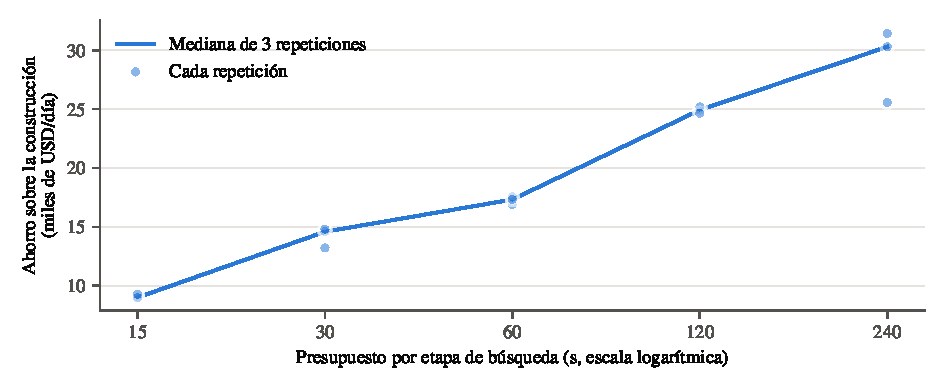
\includegraphics[width=\textwidth]{figures/barrido.pdf}
\caption{Ahorro de la búsqueda local sobre la construcción según el presupuesto por etapa (tres repeticiones por presupuesto, en un mismo equipo).}
\label{fig:barrido}
\end{figure}

\section{Cotas inferiores y brecha}
\label{sec:cotas}

El método no garantiza el óptimo, pero dos cotas inferiores acotan cuánto podría mejorar. La primera es la simultaneidad: a las \HoraCotaSimultaneidad{} hay \CotaSimultaneidad{} corridas en curso a la vez y cada una necesita un bus distinto; el modelo usa \BrechaBusesSimultaneidad\,\% más buses. La segunda es el flujo relajado de la fase~1 del prototipo (capítulo~\ref{ch:evolucion}), que usa los mismos sectores, ignora la batería y se resolvió a optimalidad: \FlotaFaseUno{} buses y USD~\PisoFaseUno{} al día en flota y kilómetros. Como relaja la batería, ningún plan factible con esos sectores puede costar menos. El modelo queda \BrechaCostoPiso\,\% sobre ese piso en costo y \BrechaBusesFaseUno\,\% en buses, de modo que, dentro de la sectorización, su distancia al óptimo es a lo más de \BrechaCostoPiso\,\%. Una cota no necesita ser factible para servir: basta con que ninguna solución factible pueda estar por debajo de ella.

\section{Validez de los indicadores}
\label{sec:validez-kpis}

Los buses utilizados y el costo total distinguen claramente entre el caso base y el modelo y son los que deben guiar la decisión. Los kilómetros en vacío explican parte del costo de kilómetros y muestran el efecto de compartir buses entre rutas. El uso de los electroterminales revela qué recurso limita (las plazas y no los cargadores), así que sirve para decisiones de infraestructura. Los kilómetros de servicio, en cambio, son idénticos en ambos planes (\KmServicio~km), porque dependen solo de las corridas: son un dato del problema y no un indicador. La energía comprada solo es comparable con el ajuste por la energía final, por lo que queda como indicador de apoyo, igual que el tiempo de cómputo.

\section{Limitaciones y mejoras posibles}
\label{sec:limitaciones-resultados}

Los resultados valen para un día laboral aislado, que parte con las baterías llenas y no exige reponerlas al final; esa es la principal limitación y se discute en el capítulo~\ref{ch:supuestos}. La búsqueda terminó por presupuesto y no explora intercambios entre sectores, que hoy están fijos. Tampoco se cobran las esperas, aunque con el costo de espera del enunciado la ventaja del modelo se mantiene en \DeltaPctCostoConEspera\,\% (capítulo~\ref{ch:supuestos}). Las mejoras más directas para la entrega final son dar más presupuesto a la búsqueda o mejorar la construcción, que explica la mayor parte del ahorro; permitir jornadas que crucen sectores, y exigir un estado de carga al final del día.
